\section{Introduction to Linear Programming}
\label{sect:intro-to-lp}
\begin{enumerate}
\item MATH3901 is about \emph{linear programming} (LP), a special type of
optimization problem which, as you would expect, involves ``linear'' things
only.  While only linearity is allowed in LP, it is still quite flexible and
can be applied in many real-life situations, e.g., factory productions
\faIcon{cheese}, military plannings \faIcon{bomb} (this is indeed a major
motivation for developments in LP!), etc.

\item Due to the linear nature, linear programming problems are well-studied
and many efficient approaches for solving them have already been developed.  A
natural question is then, \emph{why} are we still studying linear programming
when many performant LP solvers are available (e.g., in common coding languages
like Python)? A possible answer is that while computer \faIcon{desktop} can
assist you to solve LP problems efficiently, the responsibility of
\emph{formulating the right LP problem} (``asking the right question'') and
\emph{using the tools properly} (easier said than done!) still lies upon the
user (you!), so it is still important to understand the theoretical aspects of
linear programming and how the algorithms for solving LPs work.

Because of that, instead of focusing on what computers can do very well
(performing the often tedious computations for solving LPs), here we will
emphasize more on the \emph{conceptual} and \emph{theoretical} aspects of LPs
and the study of \emph{algorithms} for solving LPs. \begin{note} But here we
will still solve some relatively ``simple'' LP problems that require few
computations, to better understand the concepts and algorithms.
\end{note}
\end{enumerate}
\subsection{Basic Concepts in Linear Programming}
\label{subsect:lp-basic-cocnepts}
\begin{enumerate}
\item Of course, the first thing we should do is to \emph{define} what a linear
programming problem is. As suggested earlier, it is an \defn{optimization
problem}, which can be expressed as follows in general:
\begin{align*}
\text{min/max}\quad&f(\vect{x}) \\
\text{subject to (s.t.)}\quad&\vect{x}=(x_1,\dotsc,x_n)\in S
\end{align*}
where:
\begin{itemize}
\item \(f:S\to\R\) is the \defn{objective function};
\item \(S\subseteq \R^n\) is the \defn{feasible region}, and every \(\vect{x}\in S\) is called a \defn{feasible solution} or \defn{feasible point};
\item \(f^*=\inf/\sup\{f(\vect{x}):\vect{x}\in S\}\) is the \defn{optimal
value} (always unique, if exists), and \emph{every}
\(\vect{x}^{*}\in S\) with \(f(\vect{x}^{*})=f^{*}\) is called an
\defn{optimal solution} (not unique in general!).
\begin{note}
We use \(\inf/\sup\) rather than \(\min/\max\) in the definition of optimal
value to allow for more flexibility, e.g., for a minimization problem, if the
objective function is not bounded below on \(S\), ``\(\inf\)'' would give
\(-\infty\) while ``\(\min\)'' would not exist. Note that in such case, while
we have a ``\(-\infty\)'' optimal value, no optimal solution actually exists.
\end{note}
\end{itemize}
An optimization problem is said to be \defn{feasible} if the feasible region is
nonempty. The variables \(x_1,\dotsc,x_n\) are called \defn{decision
variables}.  Decision variables that are not involved in any constraints
(coming from feasible region) are known as \defn{free variables}. The primary
goal is to \emph{solve} optimization problems, i.e., finding optimal solutions
together with the optimal value (if exists).

All vectors in MATH3901 are assumed to be \emph{column vectors} unless
otherwise specified. For convenience in notations, we shall denote the column
vector \(\vect{x}= \begin{bmatrix}x_1&\cdots&x_n\end{bmatrix}^{T}\) by
\((x_1,\dotsc,x_n)\) if the entries are to be emphasized.

\item \textbf{Defining LP problems.}
Here we shall only focus on the special case where (i) the objective function
\(f\) is \underline{linear} and (ii) the feasible region \(S\) is described by
\emph{finitely many} \underline{linear} equalities or (weak)
inequalities\footnote{Allowing \emph{infinitely many} linear equalities or
inequalities would give us so much flexibility that even \emph{nonlinear}
constraints can be described!}, which is known as a \defn{linear programming
problem}:
\begin{align*}
\text{min/max}\quad&f(\vect{x})=\vect{c}^{T}\vect{x}=c_1x_1+\dotsb+c_nx_n \\
\text{s.t.}\quad&\vect{a}_j^{T}\vect{x}\le/=/\ge b_j \text{ for all \(j=1,\dotsc,m\)}
\end{align*}
where \(\vect{c},\vect{a}_1,\dotsc,\vect{a}_m\in\R^n\) and \(b_1,\dotsc,b_m\in\R\).
Here the feasible region can be expressed as \(S=\{\vect{x}\in\R^n:\vect{a}_j^{T}\vect{x}\le/=/\ge b_j\text{ for all \(j=1,\dotsc,m\)}\}\).
\begin{note}
For discussions on general optimization problems, see MATH3904.
\end{note}

\item \textbf{Examples of LP problems.}
\begin{enumerate}[label={(\arabic*)}]
\item \begin{align*}
\text{min}\quad&2x_1+3x_2-x_3 \\
\text{s.t.}\quad&x_1+2x_4\le 3\\
\quad&x_2+x_3+x_4=1 \\
\quad&x_1+x_3-2x_4\ge -2 \\
\quad&x_1,x_2,x_4\ge 0 \\
\quad&x_3\le 0
\end{align*}
\begin{note}
Here we have \(\vect{c}=(2,3,-1,0)\), \(\vect{a}_1=(1,0,0,2)\), \(b_1=3\), etc.
\end{note}
\item \begin{align*}
\text{min}\quad&x_1-x_2 \\
\text{s.t.}\quad&x_1+x_2+x_3=1\\
\quad&2x_2-3x_3=4 \\
\quad&x_1,x_2,x_3\ge 0
\end{align*}
\end{enumerate}
We can see that the second example is somewhat ``simple'' as the only
inequality constraints are for nonnegativity of \(x_1\), \(x_2\), and \(x_3\),
which are quite ``simple'' and the rest are only \emph{equality} constraints.
On the other hand, the first one involves some more complicated inequality
constraints and thus appears to be harder to deal with. In fact, the second LP
problem is in the so-called \emph{standard form}, a ``nice'' form of LP problem
that is easy to solve.

\item \textbf{Standard form of LP problems.} A LP problem is in \defn{standard
form} if it takes the following form:
\begin{align*}
\text{min}\quad&\vect{c}^{T}\vect{x} \\
\text{s.t.}\quad&A\vect{x}=\vect{b} \\
&\vect{x}\ge \vect{0}
\end{align*}
where \(\vect{c}\in\R^n\), \(A\in\R^{m\times n}\) (an \(m\times n\) matrix with
real entries), and \(\vect{b}\in\R^m\).

\begin{remark}
\item Here, \(\vect{x}\ge \vect{0}\) carries the componentwise meaning, i.e.,
\(x_1,\dotsc,x_n\ge 0\).
\item \(A\vect{x}=\vect{b}\) collects all possible \emph{equality} constraints
on the decision variables \(x_1,\dotsc,x_n\). To see this, we can identify the
\(j\)th row of \(A\) as \(\vect{a}_j^{T}\), and write
\(\vect{b}=(b_1,\dotsc,b_m)\), Then, \(A\vect{x}=\vect{b}\) just refers to the
following system of linear equations:
\[
\begin{cases}
\vect{a}_1^{T}\vect{x}=b_1 \\
\vect{a}_2^{T}\vect{x}=b_2 \\
\qquad\vdots \\
\vect{a}_m^{T}\vect{x}=b_m \\
\end{cases}
\]
\end{remark}

\item \textbf{Equivalence between optimization problems.} While not every LP is in
standard form (of course!), it turns out that it is always possible to
\emph{transform} a LP problem into a LP problem \emph{in standard form} such
that the two LP problems are \emph{equivalent}.

In general, two optimization problems of minimization\footnote{By adding a
negative sign to the objective function if necessary, we can always convert a
maximization problem to a minimization problem. Hence it suffices to focus on
optimization problems of minimization.} are said to be \defn{equivalent} if
given an \emph{arbitrary} feasible solution to \emph{each} problem, one can
construct a feasible solution to the \emph{other} system, \emph{with the same
objective value}.
\begin{note}
Sometimes, ``equivalent'' refers to the following weaker notion: Given an
arbitrary \underline{optimal} solution to each problem, one can construct an
\underline{optimal} solution to the other system, with the same
\underline{optimal} value. Often this type of equivalence is enough for the
purpose of solving optimization problems.
\end{note}

More specifically, to show that two optimization problems (A) and (B) are
equivalent, we need to carry out the following two-step process:
\begin{enumerate}[label={(\arabic*)}]
\item \emph{\(\text{(A)}\to\text{(B)}\):} Fix any feasible solution
\(\vect{x}_{A}\) to (A). Based on it, construct a solution
\(\vect{x}_A'=u(\vect{x}_A)\) such that:
\begin{enumerate}
\item \(\vect{x}_A'\) is a feasible solution to (B).
\item
\(\operatorname{obj}_{(A)}(\vect{x}_A)=\operatorname{obj}_{(B)}(\vect{x}_A')\)
where \(\operatorname{obj}_{(A)}\) and \(\operatorname{obj}_{(B)}\) are the objective functions for (A) and (B) respectively.
\end{enumerate}
\item \emph{\(\text{(B)}\to\text{(A)}\):} Fix any feasible solution
\(\vect{x}_{B}\) to (B). Based on it, construct a solution
\(\vect{x}_B'=v(\vect{x}_B)\) such that:
\begin{enumerate}
\item \(\vect{x}_B'\) is a feasible solution to (A).
\item \(\operatorname{obj}_{(A)}(\vect{x}_B')=\operatorname{obj}_{(B)}(\vect{x}_B)\).
\end{enumerate}
\end{enumerate}
We can then see that the key \faIcon{key} for showing the equivalence is to
figure out what the mappings \(u\) and \(v\) should be.

\begin{center}
\begin{tikzpicture}
\draw[] (0,0) rectangle (2,2);
\node[] () at (1,1) {(A)};
\draw[] (4,0) rectangle (6,2);
\node[] () at (5,1) {(B)};
\draw[-Latex] (1,2.5) to[bend left] node[auto]{\(u\)} (5,2.5);
\draw[-Latex] (5,-0.5) to[bend left] node[auto]{\(v\)} (1,-0.5);
\node[] () at (1,2.2) {\(\vect{x}_A\)};
\node[] () at (5,2.2) {\(\vect{x}_A'\)};
\node[] () at (1,-0.2) {\(\vect{x}_B'\)};
\node[] () at (5,-0.2) {\(\vect{x}_B\)};
\end{tikzpicture}
\end{center}

To understand this better, let us consider a simple example about proving the
equivalence between the following two LP problems (A) and (B):

(A): \begin{align*}
\text{min}\quad&x_1 \\
\text{s.t.}\quad&x_1+x_2\le 1\\
\quad&x_1,x_2\ge 0
\end{align*}

(B): \begin{align*}
\text{min}\quad&x_1 \\
\text{s.t.}\quad&x_1+x_2+x_3=1\\
\quad&x_1,x_2,x_3\ge 0
\end{align*}

\begin{pf}
Fix any feasible solution \(\vect{x}=(a,b)\) to (A). Then, consider the
solution \((x_1,x_2,x_3)=(a,b,1-a-b)\) to (B). It is feasible for (B) because
\(1-a-b\ge 0\) (and \(a,b\ge 0\) follows from the feasibility of solution for
(A)), and \(x_1+x_2+x_3=a+b+(1-a-b)=1\). Also, as these two solutions have the
same first entry, they have the same objective value \(a\) in either LP problem.

Now fix any feasible solution \(\vect{x}=(a,b,c)\) to (B). It is easy to see
that the solution \((x_1,x_2)=(a,b)\) is feasible for (A), since \(a+b\le
a+b+c=1\) (as \(c\ge 0\)) and \(a,b\ge 0\). Besides, these two solutions again
have the same first entry, hence same objective value.
\end{pf}

\item \textbf{Same optimal values for two equivalent optimization problems.}
\begin{proposition}
\label{prp:equiv-optim-same-optim}
Two equivalent optimization problems of minimizations always have the same
optimal values.
\end{proposition}
\begin{pf}
First, let us express the two optimization problems as:

(P):
\begin{align*}
\text{min}\quad&f(\vect{x}) \\
\text{s.t.}\quad&\vect{x}\in A
\end{align*}

(Q):
\begin{align*}
\text{min}\quad&g(\vect{y}) \\
\text{s.t.}\quad&\vect{y}\in B
\end{align*}

Let \(f^*\) and \(g^*\) denote the optimal values of (P) and (Q) respectively,
with \(\vect{x}^*\in A\) and \(\vect{y}^*\in B\) being corresponding optimal
solutions (not necessarily unique). Then we can write \(f^*=f(\vect{x}^*)\) and
\(g^*=g(\vect{y}^*)\). We will prove \(f^*=g^*\) by showing (i) \(f^*\le g^*\) and
(ii) \(g^*\le f^*\).

\begin{itemize}
\item \underline{\(f^*\le g^*\):} As \(\vect{y}^*\in B\), by the equivalence,
there is a mapping \(v\) such that \(v(\vect{y}^*)\in A\) and
\(f(v(\vect{y}^*))=g(\vect{y}^*)=g^*\). Thus,
\(f^*=f(\vect{x}^*)\overset{\text{(\(\vect{x}^*\) optimal)}}{\le}
f(v(\vect{y}^*)) =g^* \).
\item \underline{\(g^*\le f^*\):} As \(\vect{x}^*\in A\), by the equivalence,
there is a mapping \(u\) such that \(u(\vect{x}^*)\in B\) and
\(g(u(\vect{x}^*))=f(\vect{x}^*)=f^*\).  Thus,
\(g^*=g(\vect{y}^*)\overset{(\text{\(\vect{y}^*\) optimal})}{\le}
g(u(\vect{x}^*))=f^*\).
\end{itemize}
\end{pf}

\begin{note}
We can see that the weaker notion of ``equivalence'' suggested earlier
(concerning only optimal solutions) is indeed enough for guaranteeing the
equality between optimal values.  This also explains why this weaker notion is
often already enough for many situations.
\end{note}
\item\label{it:reduce-to-std-form} \textbf{Reducing LP problems to standard form.}
\Cref{prp:equiv-optim-same-optim} suggests a handy approach to solve LP problem,
namely by converting/reducing it to an \emph{equivalent} standard form LP
problem, and solve the latter problem instead of the original, which can be
done easily in general (many efficient algorithms are available). This approach
allows us to:
\begin{itemize}
\item obtain the optimal value (if exists) readily from the latter LP problem
(by \Cref{prp:equiv-optim-same-optim});
\item obtain also optimal solutions in the original LP problem, by constructing
from optimal solutions in the latter LP problem (by equivalence).
\end{itemize}

\begin{center}
\begin{tikzpicture}
\node[draw] (any) at (0,0) {Any LP problem};
\node[draw] (sf) at (6,0) {Standard form LP problem};
\node[draw] (os) at (12,0) {Optimal solution};
\draw[-Latex] (any) --node[midway, above]{Reduction} (sf);
\draw[-Latex] (sf) --node[midway, above]{Algorithm} (os);
\draw[Latex-Latex] (any.south) to[bend right] node[auto, swap]{same optimal value} (sf.south);
\draw[-Latex] (os.north) to[bend right] node[auto, below=0.4cm]{construct optimal solution for original} (any.north);
\draw[-Latex, dashed] (os.south) --node[midway, below]{deduce} (4.5,-1.5);
\end{tikzpicture}
\end{center}
The following theorem proposes one systematic method for converting any LP
problem to a LP problem in standard form.

\begin{theorem}
\label{thm:to-std-form-lp}
Given any LP problem, consider the following steps.
\begin{enumerate}[label={(\arabic*)}]
\item \emph{Changing to minimization:} If necessary, convert maximization to
minimization by changing the objective function \(f\to -f\).
\item \emph{Eliminating inequality constraints:} For every inequality
constraint, introduce a \defn{slack variable} (for ``\(\le\)''
case)/\defn{surplus variable} (for ``\(\ge\)'' case) \(s_j\ge 0\) as follows:
\begin{itemize}
\item \emph{(``\(\le\)'' case)} Change \(\sum_{i=1}^{n}a_{ji}x_i\le b_j\to(\sum_{i=1}^{n}a_{ji}x_i)\vc{+s_j}=b_j\).
\item \emph{(``\(\ge\)'' case)} Change \(\sum_{i=1}^{n}a_{ji}x_i\ge b_j\to(\sum_{i=1}^{n}a_{ji}x_i)\vc{-s_j}=b_j\).
\end{itemize}
\item \emph{Eliminating free variables:} Change every free variable \(x_i\to
x_i^{+}-x_i^{-}\), where \(x_i^{+}=\begin{cases}
x_i&\text{if \(x_i>0\)}, \\
0&\text{if \(x_i\le 0\)}
\end{cases}
\) and \(x_i^{-}=\begin{cases}
0&\text{if \(x_i\ge 0\)}, \\
\rc{-}x_i&\text{if \(x_i<0\)}
\end{cases}
\) denote the \defn{positive
part} and \defn{negative part} of \(x_i\) respectively.
\end{enumerate}
Performing these steps on the given LP problem would yield a LP problem in
\emph{standard form} and \emph{equivalent} to the one from original, or
obtained after the first step (changing to minimization).
\end{theorem}
\begin{pf}
Omitted; see below for an example that illustrates the main idea.
\end{pf}

\begin{note}
After performing the steps as suggested in \Cref{thm:to-std-form-lp}, we would
get a LP problem of \emph{minimization} with only equality constraints (except
the inequality constraints about nonnegativity of decision variables), and
\emph{nonnegative} decision variables coming from three sources: (i) original
\(x_i\)'s, (ii) \(x_i^{+}\)'s and \(x_i^{-}\)'s, and (iii) slack variables
\(s_j\)'s. Thus the resulting LP problem is in standard form.
\end{note}

\item \textbf{Example of reducing LP problems to standard form.} Consider the
following LP problem:
\begin{align*}
\text{max}\quad&-x_1+3x_2 \\
\text{s.t.}\quad&x_1+x_2\ge 3\\
\quad&3x_1+2x_2=14 \\
\quad&x_1\ge 0
\end{align*}
Now we carry out the steps as indicated in \Cref{thm:to-std-form-lp}:
\begin{enumerate}[label={(\arabic*)}]
\item \emph{Changing to minimization:} Change \(-x_1+3x_2\to x_1-3x_2\) and \(\max\to\min\). (Call the resulting LP problem (A).)
\item \emph{Eliminating inequality constraints:} Introduce a surplus variable
\(x_3\ge 0\) (notation does not matter), and change \(x_1+x_2\ge 3\to
x_1+x_2\vc{-x_3}=3\) (and also add an inequality constraint \(x_3\ge 0\)).
\item \emph{Eliminating free variables:} The only free variable is \(x_2\). So
we change \emph{every} \(x_2\to x_2^{+}-x_2^{-}\) (and add inequality
constraints \(x_2^{+},x_2^{-}\ge 0\)).
\end{enumerate}
The resulting LP problem in standard form (call it (B)) is then:
\begin{align*}
\text{min}\quad&x_1-3x_2^{+}+3x_2^{-} \\
\text{s.t.}\quad&x_1+x_2^{+}-x_2^{-}-x_3= 3\\
\quad&3x_1+2x_2^{+}-2x_2^{-}=14 \\
\quad&x_1,x_2^{+},x_2^{-},x_3\ge 0
\end{align*}
While the number of decision variables goes up from 2 to 4, we have
successfully simplified the LP problem so that it can be solved by efficient
algorithms coded in computer programs.

Here, let us demonstrate how to show the LP problems (A) and (B) are
equivalent, providing some insights on the proof of \Cref{thm:to-std-form-lp}.

\begin{pf}
First fix any feasible solution \((x_1,x_2)=(a,b)\) to (A). Then, consider the
solution \((x_1,x_2^{+},x_2^{-},x_3)=(a,b^{+},b^{-},3-a-(b^{+}-b^{-}))\).
It is straightforward to check that this solution is feasible for (B) and has
the same objective value (because \(b\equiv b^{+}-b^{-}\)).

Now fix any feasible solution \((x_1,x_2^{+},x_2^{-},x_3)=(a,b,c,d)\) to (B).
Then, consider the solution \((x_1,x_2)=(a,b-c)\).  Again, it is
straightforward to check that this solution is feasible for (A) and has the
same objective value.
\end{pf}
\item\label{it:piecewise-linear-cvx-to-lp} \textbf{Reducing optimization problems to LP problems.}
While many optimization problems are not LP problems, we can indeed reduce some
of them to LP problems, allowing us to solve them efficiently (through further
reduction to standard form, say). One notable example is minimization problems
involving \emph{piecewise linear convex} objective function and ``\(\leq\)''
constraints.

\textbf{Preliminaries about convex functions.}
\begin{itemize}
\item \emph{Definition:} A function \(f:\R^n\to \R\) is \defn{convex} if for
all \(\vect{x},\vect{y}\in\R^n\) and all \(\lambda\in[0,1]\), we have
\[
f(\lambda\vect{x}+(1-\lambda)\vect{y})\le\lambda
f(\vect{x})+(1-\lambda)f(\vect{y}).
\]
\begin{center}
\begin{tikzpicture}
\begin{axis}[domain=0:5, xtick={1,4}, ytick={6,9},
xticklabels={\(x\), \(y\)}, yticklabels={\(f(x)\), \(f(y)\)}]
\addplot[blue]{(x-3)^2+2*x};
\draw[magenta] (1,6) -- (4,9);
\node[magenta] (lin) at (2,10) {\(\lambda f(x)+(1-\lambda)f(y)\)};
\draw[-Latex, magenta] (lin) -- (2.5,8);
\addplot[green, opacity=0.3, domain=1:4, line width=0.1cm]{(x-3)^2+2*x};
\node[ForestGreen] () at (4,5) {\(f(\lambda x+(1-\lambda)y)\)};
\end{axis}
\end{tikzpicture}
\end{center}
\item \emph{Property of convex functions:}
\begin{proposition}
\label{prp:max-cvx-cvx}
Let \(f_1,\dotsc,f_m:\R^n\to\R\) be convex functions. Then, their
maximum \(f(x)=\max_{i=1,\dotsc,m}f_i(\vect{x})\) is convex.
\end{proposition}
\begin{pf}
Fix any \(\vect{x},\vect{y}\in\R^n\) and any \(\lambda\in[0,1]\). Then,
\begin{align*}
f(\lambda\vect{x}+(1-\lambda)\vect{y})
&=\max_{i=1,\dotsc,m}f_i(\lambda\vect{x}+(1-\lambda)\vect{y}) \\
&\le\max_{i=1,\dotsc,m}\lambda f_i(\vect{x})+(1-\lambda)f_i(\vect{y}) \\
&\le \lambda \underbrace{\max_{i=1,\dotsc,m}f_i(\vect{x})}_{f(\vect{x})}
+(1-\lambda)\underbrace{\max_{i=1,\dotsc,m}f_i(\vect{y})}_{f(\vect{y})}.
\end{align*}
\end{pf}
\end{itemize}

\Cref{prp:max-cvx-cvx} leads us to call a function of the form
\(f(\vect{x})=\max_{i=1,\dotsc,m}(\vect{c}_i^{T}\vect{x})\) \defn{piecewise
linear convex function}.

Now, consider a minimization problem problem with piecewise linear
objective function and ``\(\leq\)'' constraint, (A):
\begin{align*}
\text{min}\quad&f(\vect{x})=\max_{i=1,\dotsc,m}\vect{c}_i^{T}\vect{x} \\
\text{s.t.}\quad&\max_{j=1,\dotsc,m}\vect{a}_j^{T}\vect{x}\le b
\end{align*}
where \(\vect{c}_1,\dotsc,\vect{c}_m,\vect{a}_1,\dotsc,\vect{a}_m\in\R^n\) and
\(b\in\R\), with \(\vect{x}=(x_1,\dotsc,x_n)\).
\begin{note}
Noting that \(|x|=\max\{x,-x\}\), this form of optimization problems includes
those ``LP-like'' problems but with absolute value signs.
\end{note}
Of course, the problem (A) itself is not a LP problem in general.  But we claim
that the problem (A) is indeed equivalent to the following LP problem (B) in
the optimal case (i.e., here we are referring to the weaker notion of
equivalence concerning only optimal solutions):
\begin{align*}
\text{min}\quad&y \\
\text{s.t.}\quad&y\ge \vect{c}_i^{T}\vect{x}\text{ for all \(i=1,\dotsc,m\)} \\
\quad&\vect{a}_j^{T}\vect{x}\le b\text{ for all \(j=1,\dotsc,m\)}
\end{align*}
\begin{note}
In the LP problem (B), we have \(n+1\) decision variables:
\(x_1,\dotsc,x_n,y\). Here we also assume optimal solutions exist.
\end{note}

\begin{pf}
Fix any optimal solution \((x_1,\dotsc,x_n)=(d_1,\dotsc,d_n)=:\vect{d}\) to
(A). Then, consider the solution
\((x_1,\dotsc,x_n,y)=(d_1,\dotsc,d_n,\max_{i=1,\dotsc,m}\vect{c}_i^{T}\vect{d})\).
It is straightforward to check that this solution is also optimal to (B), and
it has the same optimal value.

Next, fix any optimal solution \((x_1,\dotsc,x_n,y)=(d_1,\dotsc,d_n,d^*)\) to
(B).  Write \(\vect{d}=(d_1,\dotsc,d_n)\). The optimality of solution forces
that \(d^*=\max_{i=1,\dotsc,m}\vect{c}_i^{T}\vect{d}\), as the latter is the
\emph{smallest} value \(y\) that satisfies \(y\ge\vect{c}_i^{T}\vect{d}\) for
every \(i=1,\dotsc,m\). This means the optimal value for (B) is precisely
\(\max_{i=1,\dotsc,m}\vect{c}_i^{T}\vect{d}\).


We can then see that the solution \((x_1,\dotsc,x_n)=(d_1,\dotsc,d_n)\) is
optimal to (A) and has the same optimal value.
\end{pf}
\end{enumerate}
\subsection{Geometry of Linear Programming}
\label{subsect:lp-geom}
\begin{enumerate}
\item Apart from analyzing LP problems in algebraic ways like what we did in
\Cref{subsect:lp-basic-cocnepts}, another useful method is to consider LP
problems \emph{geometrically}, which can yield some valuable insights that
cannot be obtained in the algebraic approach. Often, a combination of algebraic
and geometric insights is helpful for solving LP problems! Indeed, you may have
already learnt a simple geometrical approach for solving LP problems in high
school, that involves some ``movements of lines''; let us illustrate that
approach using the following example.

\item \textbf{``High school'' way of solving LP problems.}
Consider the following LP problem:
\begin{align*}
\text{min}\quad&-x_1-x_2 \\
\text{s.t.}\quad&x_1+2x_2\le 3\\
\quad&2x_1+x_2\le 3 \\
\quad&x_1,x_2\ge 0
\end{align*}
\begin{center}
\begin{tikzpicture}
\begin{axis}[ymin=-1.8, ymax=3.8, xmin=-1.8, xmax=3.8, axis lines=middle, xlabel=\(x_1\), ylabel=\(x_2\)]
\addplot[blue, domain=0:3]{(3-x)/2};
\addplot[ForestGreen, domain=0:1.5]{3-2*x};
\node[blue] () at (2.5,1) {\(x_1+2x_2=3\)};
\node[ForestGreen] () at (1.3,2.5) {\(2x_1+x_2=3\)};
\fill[yellow, opacity=0.3] (0,0) -- (0, 1.5)  -- (1,1) -- (1.5,0) -- cycle;
\node[text width=1cm] () at (0.5,0.5) {feasible region};
\draw[-Latex, magenta] (0,0) -- (-1,-1);
\node[magenta] () at (-1,-1.4) {\(\vect{c}=(-1,-1)\)};
\addplot[magenta, domain=-2:5, dashed, opacity=0.3]{-1-x};
\addplot[magenta, domain=-2:5, dashed, opacity=0.3]{-x};
\addplot[magenta, domain=-2:5, dashed, opacity=0.3]{1-x};
\addplot[magenta, domain=-2:5, dashed]{2-x};
\draw[red, fill] (1,1) circle [radius=0.7mm];
\draw[-Latex] (2,2) -- (1.2,1.2) node[pos=-0.2]{optimal solution};
\end{axis}
\end{tikzpicture}
\end{center}
Graphically, we can ``see'' \faIcon{eye} that the
optimal solution is \((x_1,x_2)=(1,1)\) (and it is
indeed the case). Let us explain a little bit more
about what we are trying to do in the picture above.
The idea is to first express the objective function as
\(\vect{c}^{T}\vect{x}\) where \(\vect{c}=(-1,-1)\) and
\(\vect{x}=(x_1,x_2)\). Then, we plot a line
\(-x_1-x_2=d\) for some constant \(d\), and ``move'' it around. As the line is ``moved'' along the direction of \(\vect{c}\), the value of \(d\) would rise. Since the LP problem is a \emph{minimization} problem, we would like to ``move'' the line along the direction \emph{opposite to} \(\vect{c}\) as far as possible.

We can then observe that, when we move the line to the
location where \(d=2\), it intersects with the feasible region
only at a single point \rc{\(\bullet\)}. This intersection
point \((x_1,x_2)=(1,1)\) is indeed the optimal solution
since, graphically, there would no longer be any feasible
solution on the line after moving it even further (i.e., there
is not any feasible solution that would lead to an even
smaller objective).

\warn{} \textbf{Limitations.}
While this approach is intuitively appealing and simple to
carry out (that's why it is often learnt in high school!), a
major limitation is that when the number of variables gets
larger, it is almost impossible to ``visualize'' a LP problem
in this fashion and solving a LP problem in this way becomes
prohibitively difficult!

Nevertheless, solving LP problems ``smartly'' often \emph{requires} some
geometrical insights and ideas. Hence, we will explore the geometrical aspects
of LP in \Cref{subsect:lp-geom}.

Firstly, we are going to define some geometry terms that describe various
elements appearing in the picture that illustrates LP above.

\item \textbf{Polyhedra.} The concept of \emph{polyhedra} is used for
describing feasible regions. A set \(S\subseteq
\R^n\) is a \defn{polyhedron} if
\(S=\{\vect{x}\in\R^n:A\vect{x}\ge\vect{b}\}\) for some
\(A\in\R^{m\times n}\) and \(\vect{b}\in\R^m\).

In the example above, the feasible region is
\begin{align*}
S&=\{(x_1,x_2)\in\R^2:x_1+2x_2\le 3, 2x_1+x_2\le 3,
x_1\ge 0,x_2\ge 0\} \\
&=\{(x_1,x_2)\in\R^2:-x_1+-x_2\ge -3, -2x_1-x_2\ge -3,
x_1\ge 0,x_2\ge 0\} \\
&=\left\{(x_1,x_2)\in\R^2:
\begin{bmatrix}-1&-2\\ -2&-1\\ 1&0\\ 0&1\end{bmatrix}
\begin{bmatrix}x_1\\ x_2\end{bmatrix}
\ge \begin{bmatrix}-3\\ -3\\ 0\\ 0\end{bmatrix}
\right\},
\end{align*}
which is a polyhedron.
\begin{center}
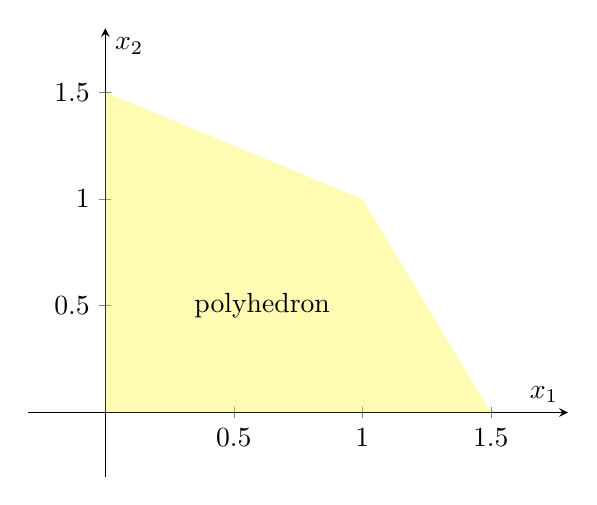
\begin{tikzpicture}
\begin{axis}[ymin=-0.3, ymax=1.8, xmin=-0.3, xmax=1.8, axis lines=middle, xlabel=\(x_1\), ylabel=\(x_2\)]
\fill[yellow, opacity=0.3] (0,0) -- (0, 1.5)  -- (1,1) -- (1.5,0) -- cycle;
\node[text width=1cm] () at (0.5,0.5) {polyhedron};
\end{axis}
\end{tikzpicture}
\end{center}
In general, the feasible region of \emph{every} LP problem is a polyhedron,
because we can always express each equality/inequality constraint in the
``\(\ge\)'' form:
\begin{itemize}
\item \(\vect{a}_j^{T}\vect{x}\ge b_j\) \cmark
\item \(\vect{a}_j^{T}\vect{x}\le b_j\to -\vect{a}_j^{T}\vect{x}\ge -b_j\)
\item \(\vect{a}_j^{T}\vect{x}= b_j\to \begin{cases}
\vect{a}_j^{T}\vect{x}\ge b_j \\
-\vect{a}_j^{T}\vect{x}\ge -b_j
\end{cases}
\)
\end{itemize}

\item \textbf{Special cases of polyhedra.} The following types of polyhedra only
involve \emph{one} equality/inequality in the condition.
\begin{itemize}
\item A set \(S\subseteq \R^n\) is a \defn{hyperplane} if
\(S=\{\vect{x}\in\R^n:\vect{a}^{T}\vect{x}=\vect{b}\}\) for some
\(\vect{a}\in\R^n\setminus \{\vect{0}\}\) and \(\vect{b}\in\R\).

\item A set \(S\subseteq \R^n\) is a \defn{halfspace} if
\(S=\{\vect{x}\in\R^n:\vect{a}^{T}\vect{x}\ge \vect{b}\}\) for some
\(\vect{a}\in\R^n\setminus \{\vect{0}\}\) and \(\vect{b}\in\R\).
\begin{center}
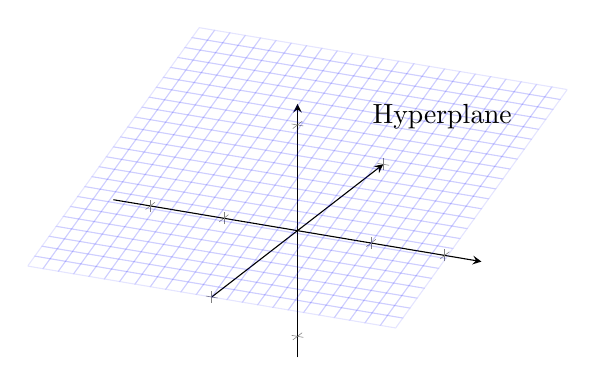
\begin{tikzpicture}
\begin{axis}[xticklabels={}, yticklabels={}, zticklabels={}, axis lines=middle, zmax=1.2, zmin=-1.2]
\addplot3[mesh, blue, opacity=0.1]{0.1*y+0.5};
\node[] () at (3,2,1) {Hyperplane};
\end{axis}
\end{tikzpicture}
\end{center}
\end{itemize}
In general, a hyperplane ``splits'' the Euclidean space \(\R^n\) into two
parts, and each of them is a \emph{halfspace} (roughly: \underline{half} of the
Euclidean \underline{space} \(\R^n\)).

Since a polyhedron \(P\) is formed by finitely many ``\(\ge\)'' constraints, we
can always express it as the \emph{intersection} of finitely many halfspaces:
\[
P=\{\vect{x}\in\R^n:A\vect{x}\ge\vect{b}\}
=\{\vect{x}\in\R^n:\vect{a}_j^{T}\vect{x}\ge b_j\text{ for all \(j=1,\dotsc,m\)}\}
=\bigcap_{j=1}^{m}\{\vect{x}\in\R^n:\vect{a}_j^{T}\vect{x}\ge b_j\}.
\]
For example, the polyhedron in the previous example is the intersection of four
halfspaces (which four?).
\begin{center}
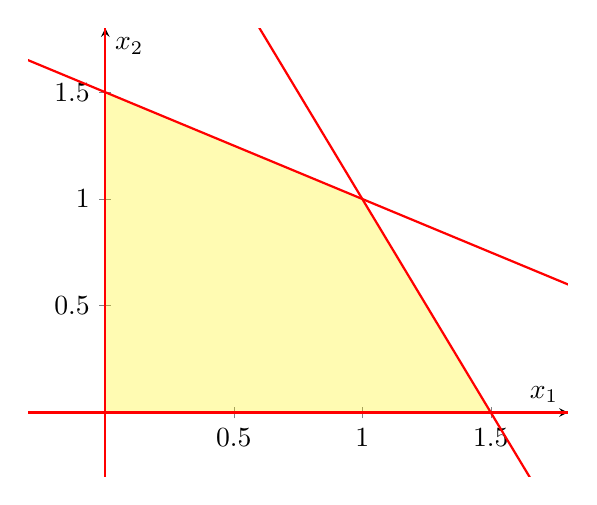
\begin{tikzpicture}
\begin{axis}[ymin=-0.3, ymax=1.8, xmin=-0.3, xmax=1.8, axis lines=middle, xlabel=\(x_1\), ylabel=\(x_2\)]
\fill[yellow, opacity=0.3] (0,0) -- (0, 1.5)  -- (1,1) -- (1.5,0) -- cycle;
\addplot[red, thick]{(3-x)/2};
\addplot[red, thick]{3-2*x};
\draw[red, thick] (0,-0.5) -- (0,2);
\draw[red, thick] (-0.5,0) -- (2,0);
\end{axis}
\end{tikzpicture}
\end{center}
\item \textbf{Convex sets.} Geometrically, we can observe that a polyhedron is
always ``bowed outward''. Mathematically, we can describe this feature via
\emph{convex set}. A set \(S\subseteq \R^n\) is \defn{convex} if for all
\(\vect{x},\vect{y}\in S\) and all \(\lambda\in[0,1]\), we have \(\lambda
\vect{x}+(1-\lambda)\vect{y}\in S\). It is not hard to see that this definition
is rather similar to that for \emph{convex function}. Indeed, a convex function
can be defined as a function whose \defn{epigraph} (i.e., the set of points
lying on or above the graph of the function) is a convex set.
\begin{center}
\begin{tikzpicture}
\begin{axis}[domain=0:5, xtick=\empty, ytick=\empty]
\addplot[blue, name path=A, thick]{(x-3)^2+2*x};
\addplot[draw=none, name path=B]{15};
\addplot[yellow, opacity=0.3] fill between[of=A and B];
\end{axis}
\end{tikzpicture}
\end{center}

Graphically speaking, a convex set contains every line segment between two
points in the set:
\begin{center}
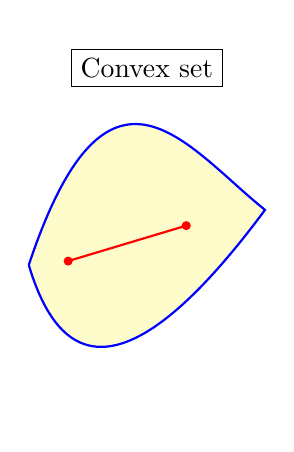
\begin{tikzpicture}
\draw[blue, fill=yellow!20!white, thick] (0,0) .. controls (1,3) and (2,1.5) .. (3,0.7) 
.. controls (1,-2) and (0.3,-1) .. (0,0);
\node[draw] () at (1.5,2.5) {Convex set};
\draw[fill, red] (0.5,0.05) circle [radius=0.5mm];
\draw[fill, red] (2,0.5) circle [radius=0.5mm];
\draw[red, thick] (0.5,0.05) -- (2,0.5);
\end{tikzpicture}
\qquad
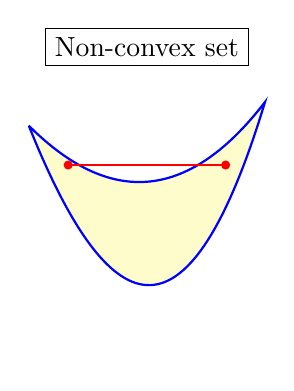
\begin{tikzpicture}
\draw[blue, fill=yellow!20!white, thick] (0,0) .. controls (1,-1) and (2,-1) .. (3,0.3) 
.. controls (2,-3) and (1,-2.5) .. (0,0);
\node[draw] () at (1.5,1) {Non-convex set};
\draw[fill, red] (0.5,-0.5) circle [radius=0.5mm];
\draw[fill, red] (2.5,-0.5) circle [radius=0.5mm];
\draw[red, thick] (0.5,-0.5) -- (2.5,-0.5);
\end{tikzpicture}
\end{center}

\item\label{it:polyhedron-cvx} Agreeing with our geometrical intuition, a polyhedron is indeed convex.

\begin{pf}
Consider any polyhedron \(P=\{\vect{x}\in\R^n:A\vect{x}\ge b\}\). Fix any
\(\vect{x},\vect{y}\in P\) and any \(\lambda\in[0,1]\). Since
\[
A(\lambda \vect{x}+(1-\lambda)\vect{y})
=\lambda A\vect{x}+(1-\lambda)A\vect{y}
\ge \lambda A\vect{b} + (1-\lambda)A\vect{b}
=A\vect{b},
\]
we have \(\lambda \vect{x}+(1-\lambda)\vect{y}\in P\), hence \(P\) is convex.
\end{pf}

\item \textbf{Vertices.} After investigating how to describe the ``bowing out''
feature of polyhedron mathematically, we will look into another geometrical
feature of a polyhedron, namely the appearance of ``corners''.
\begin{center}
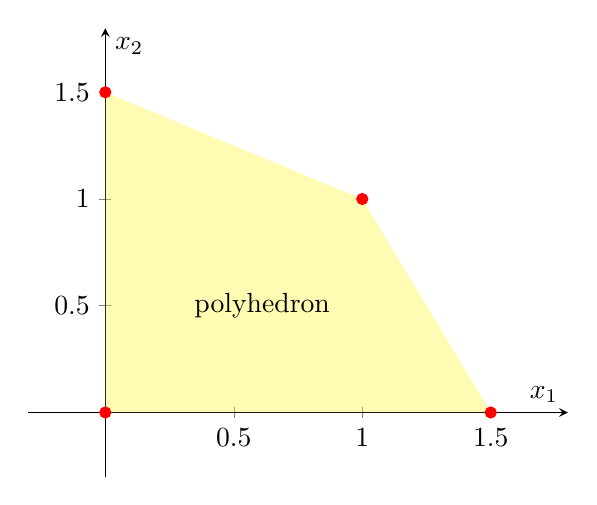
\begin{tikzpicture}
\begin{axis}[ymin=-0.3, ymax=1.8, xmin=-0.3, xmax=1.8, axis lines=middle, xlabel=\(x_1\), ylabel=\(x_2\)]
\fill[yellow, opacity=0.3] (0,0) -- (0, 1.5)  -- (1,1) -- (1.5,0) -- cycle;
\node[text width=1cm] () at (0.5,0.5) {polyhedron};
\draw[red, fill] (0,0) circle [radius=0.7mm];
\draw[red, fill] (0,1.5) circle [radius=0.7mm];
\draw[red, fill] (1,1) circle [radius=0.7mm];
\draw[red, fill] (1.5,0) circle [radius=0.7mm];
\end{axis}
\end{tikzpicture}
\end{center}
For example, for the polyhedron above, intuitively it should have four
``corners'' or \emph{vertices}, located at the \rc{red} dots in the picture;
they are some ``extreme points'' or ``tips'' of the polyhedron. But how should
we describe them mathematically?

A rather clever and tricky way to characterize the concept of \emph{vertex} is
as follows. Let \(P\) be a polyhedron. Then a point \(\vect{x}\in P\) is said
to be a \defn{vertex} of \(P\) if for all \(\vect{y},\vect{z}\in P\setminus
\{\vect{x}\}\) and all \(\lambda\in[0,1]\), we have \(\vect{x}\ne
\lambda\vect{y}+(1-\lambda)\vect{z}\).

In words, a point \(\vect{x}\) is vertex if it is \emph{not} contained in the
line segment between any two points that are both different from \(x\).  With
this definition, those \rc{red} dots above are indeed vertices of the
polyhedron, aligning with our geometrical intuition (check!).

\item \textbf{Algebraic characterization of vertices.} While the above
definition of \emph{vertex} is technically ``correct'', it is rather
inconvenient work with, because it is not clear how we can \emph{find} vertices
based on \emph{algebraic} expressions of polyhedra! Thus we would like to
characterize vertices \emph{algebraically}.

Consider a polyhedron \(P\subseteq \R^n\) with the following general expression:
\[
P=\{x\in\R^n:\vect{a}_i^{T}\vect{x}\ge b_i,~\forall i\in M_1;
\vect{a}_i^{T}\vect{x}\le b_i,~\forall i\in M_2;
\vect{a}_i^{T}\vect{x}=b_i,~\forall i\in M_3\}
\]
where \(M_1\), \(M_2\), and \(M_3\) are finite index sets. The key \faIcon{key}
for characterizing vertices algebraically is to use the idea of \emph{active
constraints}. A constraint \(\vect{a}_i^{T}\vect{x}\le/=/\ge b_i\) is
\defn{active at \(\vect{x}^*\)} if \emph{equality} is achieved at
\(\vect{x}^*\), i.e., \(\vect{a}_i^{T}\vect{x}^*=b_i\).

In the following picture, points at which some constraints are active are lying
on red lines. Our geometrical intuition then tells us that vertices are
precisely those points where \emph{many} constraints are active. But what is
meant by ``many''? To be more precise, we need to use the concept of
\emph{basic solution}.
\begin{center}
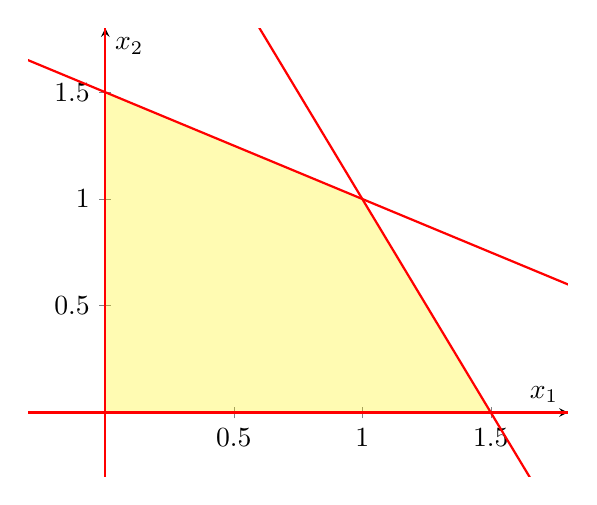
\begin{tikzpicture}
\begin{axis}[ymin=-0.3, ymax=1.8, xmin=-0.3, xmax=1.8, axis lines=middle, xlabel=\(x_1\), ylabel=\(x_2\)]
\fill[yellow, opacity=0.3] (0,0) -- (0, 1.5)  -- (1,1) -- (1.5,0) -- cycle;
\addplot[red, thick]{(3-x)/2};
\addplot[red, thick]{3-2*x};
\draw[red, thick] (0,-0.5) -- (0,2);
\draw[red, thick] (-0.5,0) -- (2,0);
\end{axis}
\end{tikzpicture}
\end{center}

\item\label{it:bfs} \textbf{Basic (feasible) solutions.} Let \(\vect{x}^*\in\R^n\). Then
\(\vect{x}^*\) is a \defn{basic solution} (of \(P\)) if (i) all equality
constraints are active at \(\vect{x}^*\), and (ii) there are \(n\) \emph{linearly
independent} constraints active at \(\vect{x}^*\).\footnote{We require linear
independence to avoid having several ``redundant'' active constraints, like
\(x_1^*+x_2^*+x_3^*=1\) and \(2x_1^*+2x_2^*+2x_3^*=2\), which are technically
``different'' but redundant.}
\begin{note}
The constraints
\(\vect{a}_{i_1}^{T}\vect{x}\ge/=/\le b_{i_1},\dotsc,\vect{a}_{i_n}^{T}\vect{x}\ge/=/\le b_{i_n}\)
are said to be linearly independent if \(\vect{a}_{i_1},\dotsc,\vect{a}_{i_n}\)
are linearly independent.
\end{note}

We also say that \(\vect{x}^*\) is a \defn{basic feasible solution} (of \(P\))
if it is a basic solution that satisfies all the constraints for \(P\) (i.e.,
is feasible).

\begin{note}
Recall from linear algebra that, for an \(n\times n\) matrix \(A\), the
following are equivalent:
\begin{enumerate}
\item Rows of \(A\) are linearly independent.
\item Columns of \(A\) are linearly independent.
\item \(\rk{A}=n\).
\item \(\det(A)\ne 0\).
\item \(A\) is invertible.
\end{enumerate}
\end{note}

The \rc{red} points below are indeed all the basic feasible solutions of \(P\),
which coincides with our usual understanding of vertices. This is in fact not a
coincidence, and being a basic feasible solution is actually \emph{equivalent}
to being a vertex.
\begin{center}
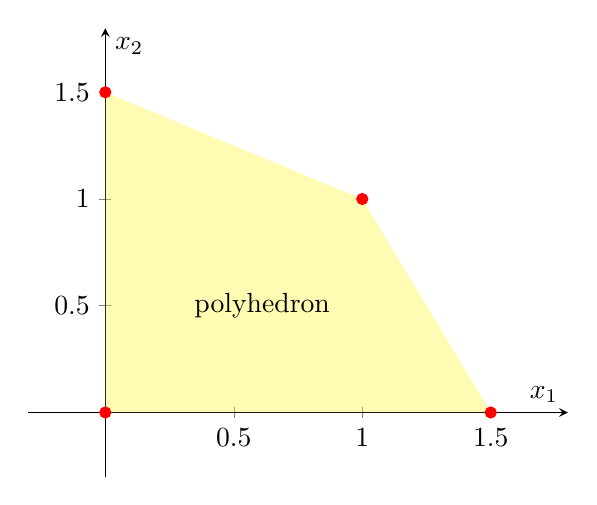
\begin{tikzpicture}
\begin{axis}[ymin=-0.3, ymax=1.8, xmin=-0.3, xmax=1.8, axis lines=middle, xlabel=\(x_1\), ylabel=\(x_2\)]
\fill[yellow, opacity=0.3] (0,0) -- (0, 1.5)  -- (1,1) -- (1.5,0) -- cycle;
\node[text width=1cm] () at (0.5,0.5) {polyhedron};
\draw[red, fill] (0,0) circle [radius=0.7mm];
\draw[red, fill] (0,1.5) circle [radius=0.7mm];
\draw[red, fill] (1,1) circle [radius=0.7mm];
\draw[red, fill] (1.5,0) circle [radius=0.7mm];
\end{axis}
\end{tikzpicture}
\end{center}

\item \textbf{Equivalent characterization of vertices.}
\begin{theorem}[Equivalent characterization of vertices]
\label{thm:vertex-equiv-bfs}
Let \(P\subseteq \R^n\) be a polyhedron and \(\vect{x}^*\in\R^n\). Then
\(\vect{x}^*\) is a vertex of \(P\) iff \(\vect{x}^*\) is a basic feasible
solution of \(P\).
\end{theorem}
\begin{pf}
``\(\Rightarrow\)'': Fix any vertex \(\vect{x}^*\) of \(P\). By definition,
\(\vect{x}^*\in P\) so it is feasible. Hence it suffices to show that it is a
basic solution of \(P\) as well.

\textbf{Introducing the set of indices for all the active constraints and direction \(\vect{d}\).}
Due to the feasibility, all equality constraints have to be active at
\(\vect{x}^*\), so it remains to show that there are \(n\) linearly independent
constraints active at \(\vect{x}^*\). Let
\(I:=\{i:\vect{a}_i^{T}\vect{x}^*=b_i\}\) denote the set of indices for
all the constraints active at \(\vect{x}^*\). Assume to the contrary that \(\spn{\{a_i:i\in
I\}}\subsetneq\R^n\). Then there is a nonzero vector
\(\vect{d}\in\R^n\) such that \(\vect{a}_i^{T}\vect{d}=0\) for all \(i\in I\)
(it originates from the orthogonal complement \(\spn{\{a_i:i\in I\}}^{\perp}\),
which is nonzero as \(\spn{\{a_i:i\in I\}}\subsetneq \R^n\)).

\textbf{Moving along the direction \(\vect{d}\) to yield contradiction.}
Next, we would like to ``move along'' the direction \(\vect{d}\) to get two
points \(\vect{y},\vect{z}\in P\setminus \{\vect{x}^*\}\) such that
\(\vect{x}^*=\lambda\vect{y}+(1-\lambda)\vect{z}\) for some
\(\lambda\in[0,1]\), leading to a contradiction.
To do that, we choose a sufficiently small \(\varepsilon>0\), and take
\(\vect{y}=\vect{x}^*+\varepsilon\vect{d}\) and \(\vect{z}=\vect{x}^*-\varepsilon\vect{d}\).
\begin{center}
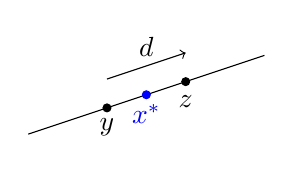
\begin{tikzpicture}
\draw[] (0,0) -- (3,1);
\draw[fill, blue] (1.5,\fpeval{1.5/3}) circle [radius=0.5mm];
\node[blue] () at (1.5,0.25) {\(\vect{x}^*\)};
\draw[fill] (1,\fpeval{1/3}) circle [radius=0.5mm];
\draw[fill] (2,\fpeval{2/3}) circle [radius=0.5mm];
\node[] () at (1,\fpeval{0.25-0.5/3}) {\(\vect{y}\)};
\node[] () at (2,\fpeval{0.25+0.5/3}) {\(\vect{z}\)};
\draw[->] (1,0.7) -- (2,\fpeval{0.7+1/3})
node[midway, above]{\(\vect{d}\)};
\end{tikzpicture}
\end{center}
To see why these choices achieve what we want, consider:
\begin{itemize}
\item \underline{\(\vect{y},\vect{z}\in P\setminus \{\vect{x}^*\}\)}:
First it is clear that \(\vect{y}\ne\vect{x}^*\) and \(\vect{z}\ne\vect{x}^*\)
as \(\vect{d}\ne\vect{0}\). Then consider two cases:
\begin{enumerate}
\item Fix any \(i\in I\). We have \(\vect{a}_i^{T}\vect{y}=
\underbrace{\vect{a}_i^{T}\vect{x}^*}_{b_i}
+\varepsilon\underbrace{\vect{a}_i^{T}\vect{d}}_{0}= b_i \), so the constraint
(``\(=\)''/``\(\le\)''/``\(\ge\)'') is satisfied by \(\vect{y}\).
\item Fix any \(i\notin I\). WLOG assume that the constraint is of the form
\(\vect{a}_i^{T}\vect{x}\ge b_i\). Since it is not active at \(\vect{x}^*\), we have
\(\vect{a}_i^{T}\vect{x}^{*}>b_i\). Thus,
\(\vect{a}_i^{T}\vect{y}=\vect{a}_i^{T}\vect{x}^*+\varepsilon\vect{a}_i^{T}\vect{d}
\overset{\text{(\(\varepsilon\) suff.~small)}}{>}b_i\). (We can choose
\(\varepsilon\) such that \(\varepsilon|\vect{a}_i^{T}\vect{d}|<\vect{a}_i^{T}\vect{x}^*-b_i\).)
So the constraint is satisfied by \(\vect{y}\).
\end{enumerate}
The argument is similar for \(\vect{z}\), and so we know \(\vect{y},\vect{z}\in
P\).
\item \underline{\(\vect{x}^*=\lambda\vect{y}+(1-\lambda)\vect{z}\) for some
\(\lambda\in[0,1]\)}: Note that \(\vect{x}^*=(1/2)\vect{y}+(1/2)\vect{z}\).
\end{itemize}
Contradiction.

Hence we have \(\spn{\{a_i:i\in I\}}=\R^n\), so from linear algebra we know
\(\{\vect{a}_i:i\in I\}\) contains \(n\) linearly independent vectors.

``\(\Leftarrow\)'': Fix any basic feasible solution \(\vect{x}^*\) of \(P\),
and let \(I=\{i:\vect{a}_i^{T}\vect{x}^*=b_i\}\). Assume to the contrary that
\(\vect{x}^*\) is not a vertex. Then there exist \(\vect{y},\vect{z}\in
P\setminus \{\vect{x}^*\}\) and \(\lambda\in[0,1]\) such that
\(\vect{x}^*=\lambda\vect{y}+(1-\lambda)\vect{z}\).

\textbf{Introducing a direction \(\vect{d}\) and expressing
\(\vect{y},\vect{z}\) in terms of it.} Let \(\vect{d}=\vect{y}-\vect{x}^*\ne
\vect{0}\). Then \(\vect{y}=\vect{x}^*+\vect{d}\) and
\(\vect{z}=\vect{x}^*-t\vect{d}\) for some \(t>0\).
\begin{center}
\begin{tikzpicture}
\draw[fill, blue] (1.5,0.5) circle [radius=0.5mm];
\node[blue] () at (1.5,0.25) {\(\vect{x}^*\)};
\draw[fill, blue] (0.5,1) circle [radius=0.5mm];
\node[blue] () at (0.5,0.7) {\(\vect{y}\)};
\draw[->] (1.8,1.05) -- (0.8,1.5)
node[midway, above]{\(\vect{d}\)};
\draw[fill] (3,-0.25) circle [radius=0.5mm];
\node[] () at (3,-0.55) {\(\vect{z}\)};
\end{tikzpicture}
\end{center}
\textbf{Obtaining a contradiction by considering \(\vect{a}_i^{T}\vect{y}\) and
\(\vect{a}_i^{T}\vect{z}\).}
Since \(\vect{x}^*\) is a basic feasible solution of \(P\), \(\{\vect{a}_i:i\in I\}\)
contains \(n\) linearly independent vectors, thus \(\spn{\{\vect{a}_i:i\in
I\}}=\R^n\). This means there exists \(i\in I\) such that
\(\vect{a}_i^{T}\vect{d}\ne 0\) (as it is not possible to have a
\emph{nonzero} \(\vect{d}\) with \(\vect{a}_i^{T}\vect{d}=0~\forall i\in I\)).
WLOG, assume \(\vect{a}_i^{T}\vect{d}>0\). Then,
\[
\vect{a}_i^{T}\vect{y}=\underbrace{\vect{a}_i^{T}\vect{x}^*}_{b_i}
+\underbrace{\vect{a}_i^{T}\vect{d}}_{>0}
>b_i\text{,\quad while\quad}
\vect{a}_i^{T}\vect{z}=\underbrace{\vect{a}_i^{T}\vect{x}^*}_{b_i}
-\underbrace{t\vect{a}_i^{T}\vect{d}}_{>0}
<b_i.
\]
This suggests that it is impossible for \(\vect{y}\) and \(\vect{z}\) to
satisfy this constraint simultaneously, thus \(\vect{y}\notin P\) or
\(\vect{z}\notin P\), contradiction.
\end{pf}

\item \textbf{Specialized characterization of basic solutions for standard form
polyhedra.} For \emph{standard form} polyhedra
\(P=\{\vect{x}\in\R^n:A\vect{x}\ge\vect{b},\vect{x}\ge\vect{0}\}\)
(corresponding to standard form LP problems), we have a specialized
characterization for basic (feasible) solution, which will be helpful in the
development of the \emph{simplex method} in \Cref{sect:simplex-method}.
Recall from \labelcref{it:bfs} that, for a general polyhedron \(P\subseteq
\R^n\), \(\vect{x}^*\in\R^n\) is called a basic solution of \(P\) if (i) all equality
constraints are active at \(\vect{x}^*\), and (ii) there are \(n\) \emph{linearly
independent} constraints active at \(\vect{x}^*\). Here we will derive
an alternative characterization for a \emph{standard form} polyhedron, and the
following lemma will be helpful for the proof.
\begin{lemma}
\label{lma:n-li-active-iff-unique-sol}
Let \(\vect{x}^*\in\R^n\) and let \(I=\{i:\vect{a}_i^{T}\vect{x}=b_i\}\) be the
set of indices of constraints that are active at \(\vect{x}^*\).  Then there
are \(n\) linearly independent vectors in the set \(\{\vect{a}_i:i\in I\}\) iff
the system of equations \(\vect{a}_i^{T}\vect{x}=b_i~\forall i\in I\) has a
unique solution.
\end{lemma}
\begin{pf}
``\(\Rightarrow\)'': Assume there are \(n\) linearly independent vectors in the
set \(\{\vect{a}_i:i\in I\}\). Then we know that \(\spn{\{\vect{a}_i:i\in
I\}}=\R^n\). Now assume to the contrary that the system
\(\vect{a}_i^{T}\vect{x}=b_i~\forall i\in I\) has two distinct solutions
\(\vect{x}_{1}\) and \(\vect{x}_{2}\). Then for the \emph{nonzero} vector
\(\vect{d}=\vect{x}_1-\vect{x}_2\), we have \(\vect{a}_i^{T}\vect{d}=0\) for
all \(i\in I\), contradicting to \(\spn{\{\vect{a}_i:i\in I\}}=\R^n\).

``\(\Leftarrow\)'': Assume the system of equations
\(\vect{a}_i^{T}\vect{x}=b_i~\forall i\in I\) has a unique solution.  Due to
the uniqueness, it is not possible to have a nonzero vector \(\vect{d}\) with
\(\vect{a}_i^{T}\vect{d}=0~\forall i\in I\). Thus, the orthogonal complement is
\(\{\vect{a}_i:i\in I\}^{\perp}=\spn{\{\vect{a}_i:i\in I\}}^{\perp}=\{\vect{0}\}\),
which implies that \(\spn{\{\vect{a}_i:i\in I\}}=\R^n\). By the reduction
approach from linear algebra, we know \(\{\vect{a}_i:i\in I\}\) contains \(n\)
linearly independent vectors.
\end{pf}
\begin{theorem}
\label{thm:std-form-basic-sol}
Let \(P=\{\vect{x}\in\R^n:A\vect{x}=\vect{b}, \vect{x}\ge\vect{0}\}\) be a
standard form polyhedron, where \(A\in\R^{m\times n}\) and \(\vect{b}\in\R^m\).
Suppose that the \(m\) rows of \(A\) are linearly independent (which implies
that \(m\le n\)). Then \(\vect{x}=(x_1,\dotsc,x_n)\in\R^n\) is a basic solution
of \(P\) iff (i) there exist \(m\) linearly independent columns
\(\vect{A}_{B(1)},\dotsc,\vect{A}_{B(m)}\) of \(A\) such that
\(\sum_{i=1}^{m}\vect{A}_{B(i)}x_{B(i)}=\vect{b}\), and
(ii) \(x_{N(1)}=\dotsb=x_{N(n-m)}=0\) where
\(\{N(1),\dotsc,N(n-m)\}=\{1,\dotsc,n\}\setminus \{B(1),\dotsc,B(m)\}\).
\end{theorem}
\begin{pf}
``\(\Leftarrow\)'': Consider a \(\vect{x}\in\R^n\) and assume that (i) and (ii)
hold. Then we have
\(A\vect{x}=\sum_{i=1}^{m}\vect{A}_{B(i)}x_{B(i)}=\vect{b}\), so the equality
constraints are satisfied. Since the vectors
\(\vect{A}_{B(1)},\dotsc,\vect{A}_{B(m)}\) are linearly independent, the
variables \(x_{B(1)},\dotsc,x_{B(m)}\) must be uniquely determined: If we have
\(\sum_{i=1}^{m}\vect{A}_{B(i)}\widetilde{x}_{B(i)}=\vect{b}\), then
subtracting this from the equation above gives
\(\sum_{i=1}^{m}\vect{A}_{B(i)}(x_{B(i)}-\widetilde{x}_{B(i)})=\vect{0}\),
which implies by the linear independence that \(\widetilde{x}_{B(i)}=x_{B(i)}\)
for all \(i=1,\dotsc,m\).

Since the other variables are always zero, the system \(A\vect{x}=\vect{b}\)
has also a unique solution. Thus, by \Cref{lma:n-li-active-iff-unique-sol}, we
know there are \(n\) linearly independent constraints active at \(\vect{x}\).

``\(\Rightarrow\)'': Assume that \(\vect{x}\in\R^n\) is a basic solution. Let
\(x_{B(1)},\dotsc,x_{B(k)}\) be the \emph{only} nonzero variables in
\(\vect{x}\), i.e., they are nonzero and \(x_i=0\) for all
\(i\notin\{B(1),\dotsc,B(k)\}\). Then all the active equality constraints are
given by:
\begin{itemize}
\item \(\sum_{i=1}^{k}\vect{A}_{B(i)}x_{B(i)}=\vect{b}\),
\item \(x_i=0\) for all \(i\notin\{B(1),\dotsc,B(k)\}\).
\end{itemize}
Since there are \(n\) linearly independent active ones here, we know that the
system of these equations has a unique solution by
\Cref{lma:n-li-active-iff-unique-sol}. This implies that
\(\sum_{i=1}^{k}\vect{A}_{B(i)}x_{B(i)}=\vect{b}\) has a unique solution.
Then, we know that \(\vect{A}_{B(1)},\dotsc,\vect{A}_{B(k)}\) are linearly
independent; if not, there would be \(\lambda_1,\dotsc,\lambda_k\) that are not all
zero such that \(\sum_{i=1}^{k}\vect{A}_{B(i)}\lambda_i=0\), which would then
yield \(\sum_{i=1}^{k}\vect{A}_{B(i)}(x_{B(i)}+\lambda_i)=\vect{b}\),
contradicting to the uniqueness of solution.

Since \(A\) has \(m\) linearly independent rows, its maximal number of linearly
independent columns is also \(m\). Then we deduce that \(k\le m\), and by the
extension approach from linear algebra, we can find \(m-k\) more columns of
\(A\): \(\vect{A}_{B(k+1)},\dotsc,\vect{A}_{B(m)}\), such that
\(\vect{A}_{B(1)},\dotsc,\vect{A}_{B(m)}\) are linearly independent.

Lastly, for every \(i\in\{N(1),\dotsc,N(n-m)\}\), we have
\(i\notin\{B(1),\dotsc,B(k)\}\) (as \(k\le m\)), thus by construction we must
have \(x_i=0\). This completes the proof.
\end{pf}

\begin{remark}
\item The variables \(x_{B(1)},\dotsc,x_{B(m)}\) are called \defn{basic
variables}, while the variables \(x_{N(1)}\dotsc,x_{N(n-m)}\) are called
\defn{non-basic variables}. The collection
\(\{\vect{A}_{B(1)},\dotsc,\vect{A}_{B(m)}\}\) of \(m\) linearly independent
columns of \(A\) is called a \defn{basis} of \(A\), and the matrix formed by these
columns,
\(B=\begin{bmatrix}\vect{A}_{B(1)}&\cdots&\vect{A}_{B(m)}\end{bmatrix}\in\R^{m\times
m}\), is called a \defn{basis matrix}.

\item From the proof of ``\(\Rightarrow\)'' direction, we can see that while
the non-basic variables have to be zero, the basic variables \emph{could} be
zero as well (those \(x_{B(k+1)},\dotsc,x_{B(m)}=0\)), which would yield
\emph{more than \(n\)} active constraints at a basic solution \(\vect{x}\),
since we already have \(n\) active constraints from \(A\vect{x}=\vect{b}\)
(\(m\) active constraints) and \(x_{N(1)}=\dotsb=x_{N(n-m)}=0\) (\(n-m\) active
constraints). Such basic solution with more than \(n\) active constraints (here
this is equivalent to having some basic variables being \(0\)) is called
\defn{degenerate}. Geometrically, a degenerate basic solution is at the
intersection of three of more lines in two dimensions, or at the intersection
of four or more planes in three dimensions, etc.

It turns out that degeneracy could greatly influence algorithms for LP and
cause some undesirable behaviours. As such, in most discussions on the
algorithms for LP later, we will assume that every basic feasible solution is
\emph{nondegenerate} (so all basic variables \(x_{B(1)},\dotsc,x_{B(m)}\) are
nonzero).

\item The assumption that the rows of \(A\) are linearly independent is
actually not that restrictive. In fact, if the rows of
\(A\) are linearly \emph{dependent} for a LP problem, it indicates that
(i) some equality constraints are redundant and can be removed to make the rows
linearly independent without changing the feasible region, or (ii) the feasible region is
empty (when some contradictory equality constraints are present), which makes
such LP problem not meaningful. Therefore, such assumption can be made
throughout the discussion on standard form LP problems without loss of
generality.
\end{remark}

\item \label{it:std-form-bfs-procedure} \textbf{Procedure for finding
basic feasible solutions of standard form polyhedra.} Based on
\Cref{thm:std-form-basic-sol}, we can obtain the following procedure
for finding all basic feasible solutions of any standard form polyhedron
\(P=\{\vect{x}\in\R^n:A\vect{x}=\vect{b},\vect{x}\ge\vect{0}\}\) where
\(A\in\R^{m\times n}\) and \(\vect{b}\in\R^{m}\), with rows of \(A\) being
linearly independent (implying that \(m\le n\)):
\begin{enumerate}[label={(\arabic*)}]
\item Choose \(m\) linearly independent columns \(\vect{A}_{B(1)},\dotsc,\vect{A}_{B(m)}\) of \(A\).
\item \emph{(non-basic variables)} Set \(x_i=0\) for all \(i\notin\{B(1),\dotsc,B(m)\}\).
\item \emph{(basic variables)} Solve the system of \(m\) equations
\(A\vect{x}=B\vect{x}_{B}=\vect{b}\), where
\(B:=\begin{bmatrix}\vect{A}_{B(1)}&\cdots&\vect{A}_{B(m)}\end{bmatrix} \) is
the basis matrix and \(\vect{x}_{B}:=(x_{B(1)},\dotsc,x_{B(m)})\), for the unknowns
\(x_{B(1)},\dotsc,x_{B(m)}\). \begin{note}
Since the columns \(\vect{A}_{B(1)},\dotsc,\vect{A}_{B(m)}\) are linearly
independent, the basis matrix \(B\) must be invertible, thus the system has a
unique solution.
\end{note}
\item \emph{(determining feasibility)} If \(\vect{x}\ge\vect{0}\), then a basic
feasible solution is obtained. Otherwise, the basic solution obtained is not
feasible.
\item Repeat (1)-(4) until all combinations of linearly independent columns of
\(A\) are considered.
\end{enumerate}
From this procedure, since there are at most \(\binom{n}{m}\) combinations of
linearly independent columns of \(A\), we can deduce that a standard form
polyhedron can have at most \(\binom{n}{m}\) basic feasible solutions.

\item \textbf{Existence of vertices.} A polyhedron may not have a vertex. For
example, hyperplanes and halfspaces do not have vertices. In view of this, we
are interested in investigating \emph{when} a polyhedron would have a vertex.

Intuitively, one may think that a \emph{bounded} polyhedron always have a
vertex. This is indeed true, but the boundedness is not a necessary condition
for the existence of vertex. For example, the following picture illustrates an
unbounded polyhedron with a vertex.
\begin{center}
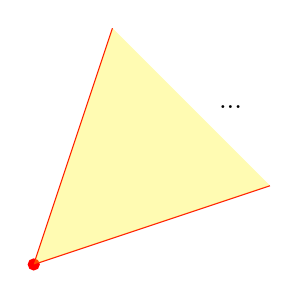
\begin{tikzpicture}
\draw[red] (0,0) -- (1,3);
\draw[red] (0,0) -- (3,1);
\draw[red, fill] (0,0) circle [radius=0.7mm];
\fill[yellow, opacity=0.3] (0,0) -- (1,3) -- (3,1) -- (0,0);
\node[] () at (2.5,2) {...};
\end{tikzpicture}
\end{center}

It turns out that a \emph{necessary} and \emph{sufficient} condition for
existence of vertices is related to whether a \emph{line} (infinitely long one;
not ``line segment'' \warn{}) is contained.

\item \textbf{Necessary and sufficient condition for existence of vertices.}
A polyhedron \(P\subseteq \R^n\) \defn{contains a line} if there exist
\(\vect{x}\in P\) and a nonzero vector \(\vect{d}\in\R^n\) such that
\(\underbrace{\vect{x}+\lambda\vect{d}}_{\mathclap{\text{point on line}}}\in P\) for all \(\lambda\in\R\).

\begin{theorem}[Necessary and sufficient condition for existence of vertices]
\label{thm:vertex-exist-noline}
A nonempty polyhedron \(P\) has at least one vertex iff it does \emph{not}
contain a line.
\end{theorem}
\begin{pf}
``\(\Rightarrow\)'': Suppose \(P\) has a vertex \(\vect{y}\), which is also a
basic feasible solution. Then there are \(n\) linearly independent constraints
active at \(\vect{y}\), say \(\vect{a}_i^{T}\vect{y}=\vect{b}_i\) for all
\(i=1,\dotsc,n\). Note that there exists \(i=1,\dotsc,n\) such that for all
nonzero vector \(\vect{d}\in\R^n\), \(\vect{a}_i^{T}\vect{d}\ne\vect{0}\);
otherwise, the orthogonal complement
\(\spn{\{\vect{a}_1,\dotsc,\vect{a}_n\}}^{\perp}\) would be nonzero and we
would have \(\spn{\{\vect{a}_1,\dotsc,\vect{a}_n\}}\subsetneq \R^n\), contradiction.

WLOG, assume the \(i\)th constraint is \(\vect{a}_i^{T}\vect{x}\ge
\vect{b}_i\). Then, for all \(\vect{x}\in P\) and all nonzero vectors
\(\vect{d}\in\R^n\), we can choose \(\lambda\) sufficiently positive/negative
(depending on the sign of \(\vect{a}_i^{T}\vect{d}\)) such that
\(\vect{a}_i^{T}(\vect{x}+\lambda\vect{d})
=\vect{a}_i^{T}\vect{x}+\lambda\vect{a}_{i}^{T}\vect{d}<b_i\), thus
\(\vect{x}+\lambda\vect{d}\notin P\). This means \(P\) does not contain a line.

``\(\Leftarrow\)'': \emph{Idea:} The following picture illustrates the key
\faIcon{key} for this part of proof: We start with an arbitrary point in
\(P\), and then keep moving along a direction such that one more ``edge'' is
touched (one more constraint becomes active) without leaving \(P\), until
reaching a vertex (basic feasible solution).
\begin{center}
\begin{tikzpicture}
\draw[blue, fill=yellow, opacity=0.3] (0,0) -- (2,1.5) -- (5,-0.5)  -- (3,-3) -- (1,-3) -- cycle;
\draw[-Latex, thick] (2.5,-1) -- (0.5,-1.5);
\draw[-Latex, thick] (0.5,-1.5) -- (1,-3);
\draw[violet, fill] (2.5,-1) circle [radius=0.7mm];
\draw[orange, fill] (0.5,-1.5) circle [radius=0.7mm];
\draw[red, fill] (1,-3) circle [radius=0.7mm];
\node[] () at (2,0.7) {\Large{\(P\)}};
\end{tikzpicture}
\end{center}
\textbf{Introducing a set of indices for active constraints.}
Assume \(P\) does not contain a line. Fix any \(\vect{x}\in P\) and let
\(I:=\{i:\vect{a}_{i}^{T}\vect{x}=b_i\}\) denote the set of indices for all the
constraints active at \(\vect{x}\). If there are \(n\) linearly independent
constraints active at \(\vect{x}\), then \(\vect{x}\) is by definition a basic
feasible solution, so a vertex of \(P\) is found.

\textbf{Moving along a direction to ``touch'' one more ``edge'' without leaving \(P\).}
So, assume henceforth that there are only \emph{less than} \(n\) linearly
independent constraints active at \(\vect{x}\). In such case, we have
\(\spn{\{\vect{a}_i:i\in I\}}\subsetneq \R^n\), and thus there is a nonzero
vector \(\vect{d}\in \R^n\) such that \(\vect{a}_i^{T}\vect{d}=0\) for all
\(i\in I\). Then consider the line \(\vect{x}+\lambda\vect{d}\) where
\(\lambda\in\R\) is the parameter.

Constraints that are active at \(\vect{x}\) are also active at every point on
this line since, for all \(i\in I\) and \(\lambda\in\R\), we have
\(\vect{a}_i^{T}(\vect{x}+\lambda\vect{d})
=\vect{a}_i^{T}\vect{x}+\lambda\vect{a}_i^{T}\vect{d}=\vect{a}_i^{T}\vect{x}+0=\vect{a}_i^{T}\vect{x}\).
This suggests that moving along the direction \(\vect{d}\) at least would not
reduce the number of ``edges touched''.

Now, we will show that it is possible to ``touch'' one more ``edge'' by
choosing an appropriate parameter \(\lambda\). By assumption, this line must
not be contained by \(P\), so as we vary the parameter \(\lambda\), some
constraints will eventually be violated. Then consider the moment at which some
constraints are about to be violated (for the first time); in such case, there
is at least one new constraint becoming active.\footnote{More formally, this
can be justified by the intermediate value theorem.} Denoting the parameter in
such case by \(\lambda^*\), we then have
\(\vect{a}_j^{T}(\vect{x}+\lambda^{*}\vect{d})=b_j\) for some \(j\notin I\) (we
have \(j\notin I\) as the constraints corresponding to indices in \(I\) would
still be active, thus not be violated for all \(\lambda\)). By construction, no
constraints are actually violated at the point \(\vect{x}+\lambda^{*}\vect{d}\)
(we just have that some constraints are \emph{about} to be violated), so
\(\vect{x}+\lambda^{*}\vect{d}\) is feasible and belongs to \(P\) still.

\textbf{Showing the linear independence of constraints with the additional one.}
To prove that \(\{\vect{a}_i:i\in I\}\cup\{\vect{a}_j\}\) is linearly
independent, it suffices to show that \(\vect{a}_j\) is a not a linear
combination of vectors in \(\{\vect{a}_i:i\in I\}\). On one hand, we have
\(\vect{a}_j^{T}\vect{x}\ne b_j\) since \(j\notin I\), and
\(\vect{a}_j^{T}(\vect{x}+\lambda^*\vect{d})=b_j\). This forces
\(\vect{a}_j^{T}\vect{d}\ne 0\). On the other hand, we know that
\(\vect{a}_i^{T}\vect{d}=0\) for all \(i\in I\), which implies that
\(\vect{a}_j\) is a not a linear
combination of vectors in \(\{\vect{a}_i:i\in I\}\); otherwise we would have
\(\vect{a}_j^{T}\vect{d}=0\)!

\textbf{Showing the existence of vertices by applying the previous argument iteratively.}
The argument above depicts a method to raise the number of active constraints
through moving to an appropriate point in \(P\). Using this method iteratively,
we will eventually reach a point in \(P\) at which \(n\) linearly independent
constraints are active; that point is the vertex we would like to find.
\end{pf}

\begin{corollary}
\label{cor:std-form-has-vertex}
Every nonempty standard form polyhedron \(P=\{\vect{x}\in\R^n:A\vect{x}=\vect{b},
\vect{x}\ge\vect{0}\}\) has at least one vertex.
\end{corollary}
\begin{pf}
Note that \(P\subseteq \{\vect{x}\in\R^n:\vect{x}\ge\vect{0}\}\) and the latter
does not contain a line. Thus \(P\) does not contain a line also, so it has at
least one vertex by \Cref{thm:vertex-exist-noline}.
\end{pf}
\item \textbf{A primer of applying geometrical concepts for solving LP
problems: optimality of vertices.}
So far we have discussed quite a lot of geometrical concepts about LP. But
ultimately, as we mention at the start, they are used for solving LP problems.
So, to illustrate how they are useful for LP problems, we will study a somewhat
simple application of geometrical concepts for solving LP problems, which is
about optimality of vertices.

This application may perhaps be learnt in high school as well. In simple terms,
it suffices to compare the values of objective functions at all the vertices,
and the smallest value is precisely the optimal value (for an minimization
problem); this method may be even more straightforward than the previous method
which involves ``moving lines''.
\begin{center}
\begin{tikzpicture}
\begin{axis}[ymin=-1.8, ymax=3.8, xmin=-1.8, xmax=3.8, axis lines=middle, xlabel=\(x_1\), ylabel=\(x_2\)]
\addplot[blue, domain=0:3]{(3-x)/2};
\addplot[ForestGreen, domain=0:1.5]{3-2*x};
\node[blue] () at (2.5,1) {\(x_1+2x_2=3\)};
\node[ForestGreen] () at (1.3,2.5) {\(2x_1+x_2=3\)};
\fill[yellow, opacity=0.3] (0,0) -- (0, 1.5)  -- (1,1) -- (1.5,0) -- cycle;
\node[text width=1cm] () at (0.5,0.5) {feasible region};
\draw[red, fill] (1,1) circle [radius=0.7mm];
\draw[red, fill] (1.5,0) circle [radius=0.7mm];
\draw[red, fill] (0,1.5) circle [radius=0.7mm];
\draw[red, fill] (0,0) circle [radius=0.7mm];
\draw[-Latex, magenta] (2,2) -- (1.2,1.2);
\draw[-Latex, magenta] (2,2) -- (1.5,0.2);
\draw[-Latex, magenta] (2,2) -- (0.2,1.5);
\draw[-Latex, magenta] (2,2) to[bend left] (0.1,0.1);
\node[magenta] () at (2.2,2.2) {compare};
\end{axis}
\end{tikzpicture}
\end{center}
In the following, we will formalize this idea and justify why this method
works.
\begin{theorem}
\label{thm:vertex-optimal}
Consider a LP problem of minimization:
\begin{align*}
\text{min}\quad&\vect{c}^{T}\vect{x} \\
\text{s.t.}\quad&\vect{x}\in P
\end{align*}
where the feasible region \(P\) is a polyhedron.  Suppose \(P\) has at least
one vertex.  Then either the optimal value is \(-\infty\)\footnote{This
corresponds to the case where the objective function is not bounded below on
\(P\).} or there exists a vertex which is an optimal solution.
\end{theorem}
\begin{pf}
\emph{Idea:} The proof strategy is similar to the one used for proving the
``\(\Leftarrow\)'' direction of \Cref{thm:vertex-exist-noline}, but we need to
ensure additionally that the values taken by the objective function do not
increase after moving to new points.

Assume \(P\) has at least one vertex. It suffices to show that any finite
optimal value is achieved at a vertex of \(P\).

\textbf{Introducing a set of indices for active constraints.} Suppose that the
optimal value is finite. Fix any point \(\vect{x}\in P\) at which there are
only \emph{less than} \(n\) linearly independent constraints that are active.
Let \(I:=\{i:\vect{a}_i^{T}\vect{x}=b_i\}\) denote the set of indices for all
the constraints active at \(\vect{x}^*\).

\textbf{Moving along a direction to ``touch'' one more ``edge'' without leaving
\(P\) or increasing the value taken by objective function.}
Since there are only \emph{less than} \(n\) linearly independent active
constraints, we have \(\spn{\{\vect{a}_i:i\in I\}}\subsetneq\R^n \), thus there
is a nonzero vector \(\vect{d}\) such that \(\vect{a}_i^{T}\vect{d}=0\) for all
\(i\in I\). By taking negative of \(\vect{d}\) if necessary, we may assume that
\(\vect{c}^{T}\vect{d}\le 0\). Now consider two cases:
\begin{itemize}
\item \emph{Case 1: \(\vect{c}^{T}\vect{d}<0\).} Consider the \emph{half-line}
\(\vect{x}+\lambda\vect{d}\) where \(\lambda\gc{\ge 0}\) is the parameter.  Like
the proof for ``\(\Leftarrow\)'' direction of \Cref{thm:vertex-exist-noline},
all the active constraints at \(\vect{x}\) are still active at every point on
this half-line, i.e., \(\vect{a}_i^{T}(\vect{x}+\lambda\vect{d})=0\) for all
\(i\in I\).

\textbf{Claim:} This half-line is not contained in \(P\).

\begin{pf}
If this half-line were contained in \(P\), the objective function
would not be bounded below on \(P\), as it can take arbitrarily negative value
on this half-line by setting arbitrarily large \(\lambda\), due to the
assumption that \(\vect{c}^{T}\vect{d}<0\). Therefore, the optimal value would
be \(-\infty\) in such case, which is impossible by our assumption at the beginning.
\end{pf}

This means that as we increase the parameter \(\lambda\ge 0\) for this half-line,
some constraints will eventually be violated. Like before, denoting by
\(\lambda^*\) the parameter for the moment at which some constraints are \emph{about}
to be violated (for the first time), we have
\(\vect{a}_j^{T}(\vect{x}+\lambda^*\vect{d})=b_j\) for some \(j\notin I\) and
\(\vect{x}+\lambda^*\vect{d}\in P\). Using a similar argument, we also know
that \(\{\vect{a}_{i}:i\in I\}\cup\{\vect{a}_j\}\) is linearly independent,
increasing the number of linearly independent active constraints by at least
one.

In addition, since \(\vect{c}^{T}\vect{d}<0\), we have
\(\vect{c}^{T}(\vect{x}+\lambda^*\vect{d})<\vect{c}^{T}\vect{x}\), meaning that
the value taken by the objective function does not increase at this new point.
\begin{center}
\begin{tikzpicture}
\draw[blue, fill=yellow, opacity=0.3] (0,0) -- (2,1.5) -- (5,-0.5)  -- (3,-3) -- (1,-3) -- cycle;
\draw[-Latex, thick] (2.5,-1) -- (0.5,-1.5);
\draw[blue] (2.5,-1) --node[pos=0.75, above=0.3cm]{half-line} (-2.5,-2.25);
\node[rotate=15, blue] () at (-2.7,-2.3) {...};
\draw[-Latex, thick] (0.5,-1.5) -- (1,-3);
\draw[ForestGreen] (0.5,-1.5) --node[pos=0.75, right=0.3cm]{half-line} (1.5,-4.5);
\node[rotate=105, ForestGreen] () at (1.55,-4.7) {...};
\draw[violet, fill] (2.5,-1) circle [radius=0.7mm];
\draw[orange, fill] (0.5,-1.5) circle [radius=0.7mm];
\draw[red, fill] (1,-3) circle [radius=0.7mm];
\node[] () at (2,0.7) {\Large{\(P\)}};
\end{tikzpicture}
\end{center}
\item \emph{Case 2: \(\vect{c}^{T}\vect{d}=0\).} Consider the line
\(\vect{x}+\lambda\vect{d}\) where \(\lambda\in\R\) is the parameter. Since
\(P\) has at least one vertex, by \Cref{thm:vertex-exist-noline} \(P\) does not
contain a line also. Thus, this line must not be contained in \(P\). Again,
like the proof for ``\(\Leftarrow\)'' direction of
\Cref{thm:vertex-exist-noline}, there exists \(\lambda^*\in\R\) such that
(i) \(\vect{a}_j^{T}(\vect{x}+\lambda^{*}\vect{d})=b_j\) for some \(j\notin I\),
(ii) \( \vect{x}+\lambda^{*}\vect{d}\in P\), and (iii) \(\{\vect{a}_{i}:i\in I\}\cup\{\vect{a}_j\}\)
is linearly independent. So this again increases the number of linearly
independent active constraints by at least one.

Furthermore, as \(\vect{c}^{T}\vect{d}=0\), we have
\(\vect{c}^{T}(\vect{x}+\lambda^{*}\vect{d})=\vect{c}^{T}\vect{x}\), meaning
that the value taken by the objective function again does not increase at this
new point.
\end{itemize}

\textbf{Showing that the optimal value is achieved at a vertex by applying the
previous argument iteratively.} Applying the argument above iteratively, we can
find a vertex/basic feasible solution \(\vect{w_x}\in P\) such that
\(\vect{c}^{T}\vect{w_{x}}\le\vect{c}^{T}\vect{x}\).  Note that there can only be finitely
many vertices/basic feasible solutions of \(P\) (as there are only finitely
many ways to choose \(n\) linearly independent constraints to be active, out of
the finitely many constraints in a LP problem), so we may denote them by
\(\vect{w}_{1},\dotsc,\vect{w}_r\).

Let \(\vect{w}^{*}\) be a vertex of \(P\) at which the objective function
takes the smallest value among all the vertices (which always exists as there
are only finitely many vertices), i.e.,
\(\vect{c}^{T}\vect{w}^{*}\le\vect{c}^{T}\vect{w}_k\) for all \(k=1,\dotsc,r\).
Note that for all \(\vect{x}\in P\): 
\begin{itemize}
\item If there are \(n\) linearly independent constraints that are active at
\(\vect{x}\), then \(\vect{x}=\vect{w}_k\) for some \(k=1,\dotsc,r\), so
\(\vect{c}^{T}\vect{w}^*\le\vect{c}^{T}\vect{w}_k=\vect{c}^{T}\vect{x}\).
\item If there are less than \(n\) linearly independent constraints that are
active at \(\vect{x}\), then by our previous argument there is a vertex \(\vect{w}_k\)
such that \(\vect{c}^{T}\vect{w_{k}}\le\vect{c}^{T}\vect{x}\) for some
\(k=1,\dotsc,r\). (The vertex \(\vect{w}_x\) must be one of the vertices
\(\vect{w}_1,\dotsc,\vect{w}_r\).) Thus, \(\vect{c}^{T}\vect{w}^*\le\vect{c}^{T}\vect{x}\).
\end{itemize}
This shows that \(\vect{c}^{T}\vect{w}^*\le\vect{c}^{T}\vect{x}\) for all
\(\vect{x}\in P\), and hence the optimal value is achieved at the vertex
\(\vect{w}^*\).
\end{pf}
\begin{corollary}
\label{cor:lp-optimal-exist}
Consider a LP problem of minimization:
\begin{align*}
\text{min}\quad&\vect{c}^{T}\vect{x} \\
\text{s.t.}\quad&\vect{x}\in P
\end{align*}
where the feasible region \(P\) is a nonempty polyhedron. Then either the
optimal value is \(-\infty\) or there exists an optimal solution.
\end{corollary}
\begin{pf}
This follows by first reducing the LP problem to an equivalent LP problem in
standard form, where the feasible region would be a polyhedron with at least
one vertex (by \Cref{cor:std-form-has-vertex}), and then applying
\Cref{thm:vertex-optimal} to such standard form LP problem.
\end{pf}

\begin{note}
Generally, for an optimization problem of minimization, it is possible that the
optimal value is not \(-\infty\), and there is also no optimal solution. For
instance, consider the optimization problem of minimizing \(1/x\) subject to
\(x\ge 1\). The optimal value is \(\inf\{1/x:x\ge 1\}=0\), but there is no
optimal solution since \(1/x>0\) for all \(x\ge 1\).
\end{note}
\end{enumerate}

